\documentclass[a4paper]{extarticle}
\usepackage[utf8]{inputenc}
\usepackage{hyperref}
\usepackage{geometry}
\usepackage{fancyhdr}
\usepackage{graphicx} % libreria per le immagini
\usepackage{amssymb} %libreria per i simboli (ex. alfabeto reco)
\usepackage{algorithm2e} %libreria per scrivere pseudocodice
\usepackage{longtable}
\usepackage{caption}
\usepackage{lastpage}
\usepackage{tabularx}
\usepackage{tcolorbox}%per teoremi e definizioni
\tcbuselibrary{theorems}
\usepackage{xcolor} %per creare colori personalizzati

%COLORS
\definecolor{mainGreenDef}{rgb}{70, 209, 49}

\setlength{\parindent}{0em}%indentazione paragrafo
\setlength{\parskip}{1em}%spazio tra paragrafi
\renewcommand{\baselinestretch}{1.3}%interlinea
\graphicspath{ {./} }
\geometry{
    a4paper,
    left=10mm,
    right=10mm,
    bottom=20mm
}


\hypersetup{
    colorlinks=true,
    linkcolor=blue,
    filecolor=blue,      
    urlcolor=blue,
    pdftitle={Overleaf Example},
    pdfpagemode=FullScreen
}

\newtcbtheorem[number within=section]{definizione}{Definizione}%
{colback=green!5,colframe=green!50!black,fonttitle=\bfseries}{th}

\newtcbtheorem[number within=section]{teorema}{Teorema}%
{colback=red!5,colframe=red!50!black,fonttitle=\bfseries}{th}

\newtcbtheorem[number within=section]{lemma}{Lemma}%
{colback=orange!5,colframe=orange,fonttitle=\bfseries}{th}

\pagestyle{fancy}
\fancyhf{}
\rhead{Federico Calò}
\lhead{Calcolabilità e Complessità}
\cfoot{  \thepage }


\title{Calcolabilità e Complessità}
\author{\href{http://www.federicocalo.it}{Federico Calò} }
\date{}

\begin{document}
\maketitle
\newpage
\tableofcontents
\voffset -30pt
\listoffigures
\listoftables

\newpage

\section*{Prefazione}

Questi sono gli appunti del corso di Calcoabilità e Complessità dell' università Aldo Moro di Bari. Come testi di referimento sono stati usati il libro "Introduzione alla teoria della computazione" di Michael Sisper e il libro "Linguaggi, modelli, complessità" di Giorgio Augello. Sono state integrate anche le slide dei docenti Pani e Covino.

Questi appunti rappresentano una personale rielaborazione dei testi citati sopra, in vista alla preparazione per il superamento dell'esame.

Si riportano in questa prefazione alcuni concetti derivanti dallo studio dell'esame di Linguaggi di Programmazione, corso tenuto dal Professore Giovanni Semeraro. Queste definizioni sono tratte dal suo libro 'Elementi di teoria dei linguaggi formali'.

\textbf{Definizione di grammatica generativa.}

Una grammatica generativa G è una quadrupla G=(X,V,S,P) ove:
\begin{itemize}
\item X è l'alfabeto terminale per la grammatica
\item V è l'alfabeto non terminale o delle variabili per la grammatica
\item S è il simbolo di partenza per la grammatica
\item P è l'insieme delle produzioni della grammatica
\end{itemize}
Inoltre devono valere le seguenti condizioni: $X\bigcap Y = \emptyset$ e $ S \in V$.

Una \textbf{grammatica libera da contesto} è una grammatica nella quale per ogni produzione $v\rightarrow w$ v è un non terminale: $\forall v \rightarrow w \in P: v \in V$

Esempio di linguaggio CF: $\{a^nb^n |n=0\}$ o $\{a^nb^{2n} | n>0\}$

Una grammatica dipendente da contesto è una grammatica in cui ogni produzione è nella forma: $yAz\rightarrow awz$ o $S\rightarrow \lambda$

\section{Introduzione}

I tre assi principali su cui si concentra questa materia sono gli automi, la computabilità e la complessità, assi collegati tra di loro da un unico fattor comune, quello di individuare le capacitò e i limiti dei calcolatori. La \textbf{complessità} riguarda lo studio del livello di computazionabilità dei problemi, ovvero si concentra sui fattori che rendono più o meno difficili i problemi da computare sotto un aspetto di vista computazionale. Durante gli anni gli studiosi hanno cercato diverse tecniche per risolvere i problemi difficile, ricercando ciò che determinava la loro difficoltà in modo da rendere il problema più facilmente risolvibile. In alcuni casi ci si deve però accontentare di una soluzione del problema non esatta, in altri casi trovare soluzioni ai problemi che sono approssimativamente esatte risulta relativamente facile. Le teorie della complessità e della \textbf{computabilità} sono strettamente correlate. Infatti nella teoria della computabilità la classificazione dei problemi è tra quelli che sono risolvibili e quelli che invece non lo sono. Molti concetti di quest'ultima teoria sono utilizzati nella teoria della complessità. Infine la \textbf{teoria degli automi} si occupa delle definizioni e delle proprietà dei modelli di calcolo matematici. Questa teoria aiuta molto la comprensione della teoria della computazione. 

\section{Linguaggi regolari}
Nella teoria della computazione si fa riferimento a diversi \textbf{modelli di computazione}, ognuno die quali è accurato in un determinato aspetto. Un primo modello sono gli automi, che hanno però un limite di memoria che possono utilizzare.

\begin{figure}[h]
\centering
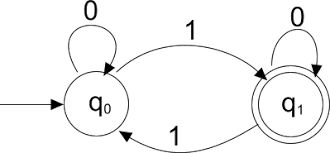
\includegraphics[scale=0.8]{Automi - Diagramma di stato}
\caption{Diagramma di Stato $M_1$}
\label{fig:1}
\end{figure}
La rappresentazione grafica di un automa prende il nome di \textbf{automa di stato}, una sua rappresentazione è definita come quella in figura 1. Ogni cerchio corrisponde a uno \textit{stato}, etichettato con un nome rappresentativo, in questo caso $q_0 e q_1$. Due componenti importanti sono lo \textit{stato di accettante}, rappresentato da due cerchi concentrici, e lo \textit{stato iniziale}, contraddistinto da una freccia entrante senza nessun label. Un ultimo elemento, che permette il passaggio da uno stato ad un altro, è costituito dalle \textit{transizioni}, rappresentate da frecce sulle quali è presente un label. Quando una stringa viene passata in input, viene prodotto un \textit{output}: accettato o rifiutato.
Un'\textbf{automa finito} è definito formalmente come una quintupla di elementi $(Q,\sum,\delta,q_0,F)$ dove:
\begin{itemize}
\item Q è un \textit{insieme di stati}
\item $\sum$ è un \textit{alfabeto}, che indica i simboli di input permessi
\item $\delta : Q \times \sum \rightarrow Q$ definita come \textit{funzione di transizione}
\item $q_0 \in Q$ definito come \textit{stato iniziale}
\item $F \subseteq Q$ definito come \textit{insieme di stati accettanti}
\end{itemize}

Se A è l'insieme di tutte le stringhe che la macchina M accetta, diciamo che A è il linguaggio della macchina M e lo rappresentiamo con la dicitura L(M)$=$A. Una macchina riconosce diverse stringhe, ma riconosce soltanto un linguaggio. Inoltre una funzione di transizione può essere descritta in forma grafica come una tabella. Facendo riferimento alla figura 1, possiamo raffigurare la relativa funzione di transizione come segue:

\begin{table}[h!]
\centering
\begin{tabularx}{0.8\textwidth} { 
  | >{\centering\arraybackslash}X 
  | >{\centering\arraybackslash}X 
  | >{\centering\arraybackslash}X | }
 \hline
   & 0 & 1 \\
 \hline
  $q_0$  & $q_0$  & $q_1$  \\
 \hline
  $q_1$ & $q_1$  & $q_0$ \\
 \hline
\end{tabularx}
\caption{Funzione di transizione della Figura 1}
\label{table:1}
\end{table}

Cerchiamo di dare una definizione formale di \textbf{computazione}. Sia $M = (Q,\sum , \delta, q_0,F)$ un automa finito e sia $w=w_1w_2...w_n$ una stringa dove ogni $w_i$ è un elemento dell'alfabeto $\sum$, allora M accetta w se esiste una sequenza  di stati $r_0,r_1,...,r_n$ in Q con tre condizioni:
\begin{itemize}
\item $r_0=q_0$
\item $\delta = (r_i,w_{i+1}=r_{i+1})$, per ogni i = 0,...,n-1
\item $r_n \in F$
\end{itemize}

Con la prima condizione si afferma che la macchina inizia dallo stato iniziale, la seconda afferma che la macchina passa da stato a stato in base alla funzione di transizione, mentre la terza afferma che la macchina accetta il suo input se termina la lettura in uno stato accettante.

\begin{definizione}{Linguaggio regolare}{theoexample}
 Un linguaggio è chiamato \textbf{linguaggio regolare} se un automa finito lo riconosce.
\end{definizione}

Come nell'aritmetica, anche nei linguaggi esistono delle operazioni che si possono applicare definite \textbf{operazioni regolari}. Diamo una definizioni di tre operazioni basilari:

\begin{definizione}{Unione, Concatenazione, Star}{theoexample}
Siano A e B due linguaggi, possiamo definire su di essi le seguenti operazioni regolari di \textbf{unione, concatenazione e star} nel seguente modo:
\begin{itemize}
\item \textbf{Unione}: $A \bigcup B = \{ x | x \in A$  oppure  $x \in B \}$
\item \textbf{Concatenazione}: A o B $= \{ xy | x \in A$ e $ y \in B \}$
\item \textbf{Star}: $A^* = \{x_1x_2...x_k|$ $k\geq 0$ e ogni $x_i \in A \}$
\end{itemize}
\end{definizione}
In poche parole l'operazione di unione unisce le stringhe dei due linguaggi in un unico linguaggio, l'operazione di concatenazione antepone le stringhe di un linguaggio ad un altro, mentre l'operazione star è l'unica operazione unaria, che opera sullo stesso linguaggio di input concatenandone le parole.

\begin{teorema} {Chiusura dell'unione}{theoexample}
La classe dei linguaggi regolari è chiusa rispetto all'operazione di unione.
\end{teorema}
Questo teorema afferma che se due linguaggi $A_1$ e $A_2$ sono regolari, lo è anche il linguaggio prodotto dalla loro unione. Questo si può dimostrare con una dimostrazione costruttiva. L'idea alla base è quella di costruire un automa M che riconosca il linguaggio $A_1 \bigcup A_2$ partendo dagli automi $M_1$ e $M_2$ che riconoscono i linguaggi $A_1$ e $A_2$.

Definiamo quindi l'automa $M_1$ come l'automa che riconosce $A_1$ composto da $M_1= (Q_1,\sum,\delta_1,q_1,F_1)$  e l'automa $M_2$ come l'automa che riconosce il linguaggio $A_2$ costituito come $M_2 = (Q_2,\sum,\delta_2,q_2,F_2)$, tramite i quali andremo successivamente a definire l'automa $M=(Q,\sum,\delta,q_0,F)$.
L'automa M quindi sarà composto come:
\begin{itemize}
\item $Q=\{ (r_1,r_2)| r_1 \in Q_1$ e  $r_2 \in Q_2\}$, insieme risultante dal prodotto cartesiano $Q_1 \times Q_2$.
\item $\sum$, l'alfabeto, che è uguale all'alfabeto dei due automi iniziali, presupponendo che i due automi abbiano lo stesso alfabeto, altrimenti sarà costituito dall'unione dei due alfabeti.
\item $\delta$, la funzione di transizione, definita per ogni $(r_1,r_2) \in Q$ e ogni $a \in \sum$, sia $\delta((r_1,r_2),a)=(\delta_1(r_1,a),\delta_2(r_2,a))$
\item $q_0$ è la coppia $(q_1,q_2)$
\item F è l'insieme costituito dall'unione degli stati finali di $M_1$ e $M_2$. Formalmente definito come $F=\{(r_1,r_2)|r_1 \in F_1$ o $r_2 \in F_2\}$.
\end{itemize}

\begin{teorema} {Chiusura della concatenazione}{theoexample}
La classe dei linguaggi regolari è chiusa rispetto all'operazione di concatenazione.
\end{teorema}

La dimostrazione di questo teorema segue la dimostrazione del teorema relativo alla chiusura di due linguaggi regolari rispetto all'unione. Infatti anche questa è una dimostrazione costruttiva, la quale parte dal presupposto che se $A_1$ e $A_2$ sono due linguaggi regolari, lo è anche la loro concatenazione. Quindi basterà costruire due automi $M_1$ e $M_2$ e concatenarli per produrre l'automa M.

Un concetto fondamentale della teoria della computazione è il concetto del \textbf{non determinismo}. Quando una macchina è in dato stato e legge il simbolo successivo, essa sa a priori qual è lo stato successivo, in quanto univocamente determinato. Si parla quindi di computazione deterministica. In una macchina non deterministica, possono esserci diverse scelte per lo stato successivo. Il determinismo è una \textit{generalizzazione} del non determinismo, quindi ogni automa finito deterministico è anche un automa finito non deterministico. Le principali differenze tra un DFA e un NFA sono abbastanza evidenti. In un DFA vi è presente sempre un arco di transizione uscente per ogni simbolo dell'alfabeto, le etichette degli archi di transizione sono sempre dei simboli dell'alfabeto. Mentre in un NFA possiamo avere archi che possono essere etichettati con $\epsilon$ e vi possono essere presenti diversi archi uscenti per uno stesso simbolo dell'alfabeto da uno stesso stato.

In un NFA il determinismo può essere visto come una computazione parallela dove processi multipli indipendenti possono essere elaborati contemporaneamente. Quando un NFA si divide per seguire diverse scelte, questo corrisponde a un processo di separazione dal processo principale, ognuno dei quali procede per conto proprio.

La formalizzazione di un automa finito non deterministico è simile a quella di un automa deterministico, la differenza principale risiede nella funzione di transizione. In un automa non deterministico, la funzione di transizione prende in input la stringa vuota o lo stato e un simbolo e produce l'insieme di possibili stati successivi. Viene così introdotto il concetto di \textbf{insieme potenza} di Q, indicato con P(Q).

Un \textbf{automa finito non deterministico} è una quintupla $(Q,\sum,\delta,q_0,F)$, dove:
\begin{itemize}
\item Q è un insieme finito di stati,
\item $\sum$ è un alfabeto finito
\item $\delta: Q\times \sum_\epsilon \longrightarrow P(Q)$ è la funzione di transizione
\item $q_0 \in Q$ è lo stato iniziale
\item $F\subseteq Q$ è l'insieme degli stati di accettazione
\end{itemize}

Nella computazione un NFA computa in maniera similare ad un DFA, con l'unica differenza per la seconda regola relativa alla funzione di transizione, la quale si trasforma in: $r_{i+1} \in \delta(r_i,y_{i+1})$, per i=0,...,m-1.

Un principio fondamentale consiste \textbf{nell'equivalenza} tra NFA e DFA, in quanto riconoscono la stessa classe di linguaggi. Ciò porta alla formalizzazione del seguente teorema
\begin{teorema}{Equivalenza tra NFA e DFA}{theoexample}
Per ogni automa finito non deterministico esiste un automa finito deterministico equivalente.
\end{teorema}

Per dimostrare questo teorema ci basta poter trasformare un NFA in un DFA che lo riconosce. Se un NFA ha un numero di stati pari a \textit{k}, significa che esso possiede un numero di sottoinsiemi di stati pari a $2^k$. Quindi dobbiamo creare una sorta di algoritmo che riesca a individuare gli stati accettanti e lo stato iniziale del DFA equivalente, e le relative transizioni. 

Per descrivere un linguaggio possiamo utilizzare delle particolari espressioni chiamate \textbf{espressioni regolari}. Definendole formalmente, un'espressione regolare può essere:
\begin{itemize}
\item a per qualche a nell'alfabeto $\sum$
\item $\epsilon$
\item $\emptyset$
\item $(R_1 \cup R_2)$, dove $R_1$ e  $R_2$ sono espressioni regolari
\item $(R_1 o R_2)$, dove $R_1$ e $R_2$ sono espressioni regolari
\item $(R_1*)$, dove $R_1$ è un'espressione regolare.
\end{itemize}
I primi due punti rappresentano i rispettivi linguaggi $\{a\}$ e $\{\epsilon\}$, mentre l'espressione regolare presente al terzo punto identifica il linguaggio che non contiene alcuna stringa. Negli altri punti invece, le espressioni regolari sono ottenute attraverso l'unione, la concatenazione o attraverso l'espressione star.

Espressioni regolari e automi finiti sono tra lo equivalenti. Possiamo enunciare un teorema che descrive questa relazione.
\begin{teorema}{Equivalenza fra automi ed espressioni regolari}{theoexample}
Un linguaggio è regolare se e solo se qualche espressione regolare lo descrive.
\end{teorema}
Introduciamo un altro tipo di automa, l'\textbf{automa finito non deterministico generalizzato} (GNA), con diverse proprietà:
\begin{itemize}
\item Lo stato iniziale ha archi di transizione uscenti verso un qualsiasi altro stato ma nessun arco entrante.
\item Esiste un solo stato accettante con archi di transizione in entrata e nessuno in uscita
\item Eccetto per lo stato iniziale e lo stato accettante, un arco va da ogni stato ad ogni altro stato e anche da ogni stato in sè stesso
\end{itemize}
Formalmente un GFA può essere definito come una quintupla $(Q,\sum,\delta,q_{start},q_{accept})$, dove:
\begin{itemize}
\item Q è l'insieme finito degli stati
\item $\sum$ è l'alfabeto di input 
\item $\delta:\{ Q-\{q_{accept}\})\times (Q-\{q_{start}) \longrightarrow R$ è la funzione di transizione
\item $q_{start}$ è lo stato iniziale
\item $q_{accept}$ è lo stato accettante   
\end{itemize}

Per dimostrare che un linguaggio è regolare, si utilizza un teorema che prende il nome di \textbf{pumping lemma}, che si basa su una proprietà particolare di tali linguaggi, secondo la quale tutte le stringhe del linguaggio possono essere replicate se la loro lunghezza raggiunge almeno un valore speciale chiamato lunghezza del pumping.

\begin{teorema}{Pumping lemma linguaggi regolare}{theoexample}
Se A è un linguaggio regolare, allora esiste un numero p (la lunghezza del pumping) tale che se s è una qualsiasi stringa in A di lunghezza almeno p, allora s può essere divisa in tre parti, s=xyz, soddisfacenti le seguenti condizioni:
\begin{itemize}
\item per ogni $i\geq0$, $xy^iz \in A$
\item $|y|>0$
\item $|xy| \leq p$
\end{itemize}
\end{teorema}

L'idea alla base per la dimostrazione di questo teorema è che se una stringa presente nel linguaggio A ha lunghezza almeno p, dobbiamo considerare la sequenza di stati che sono attraversati dalla stringa nell'automa M. Se finiamo la stringa in uno stato e la stringa è in A, sappiamo che l'ultimo stato è uno stato accettante. Se invece la lunghezza della stringa è più grande di p, allora uno stato si ripete. 

In un linguaggio più formale possiamo dimostrare il teorema 2.5.
Per la dimostrazione occorre:
\begin{itemize}
\item un DFA $M=(Q,\sum,\delta,q_1,F)$ che riconosce A
\item p, definito come un numero rappresentante il numero di stati in M
\item una stringa $s=s_1s_2...s_n$ in A di lunghezza n, dove però $n\geq p$
\item una sequenza di stati attraversati da M mentre elabora s:$r_1,r_2,...,r_{n+1}$, da cui si desume che $r_{i+1}=\delta (r_i,s_i)$ per $1\leq i\geq n$
\end{itemize}

La sequenza di stati ha una lunghezza pari a n+1, che è almeno p+1. All'interno della sequenza ci devono essere due stati che si ripetono. Possiamo denominare il primo con $r_j$ e il secondo con $r_l$- Dato che $r_l$ si ripete nelle prime p+1 posizioni in una sequenza che inizia in $r_l$, abbiamo $l\leq p+1$.

Definiamo a questo punto le tre sottostringhe che si generano: $x=s_1...s_{j-1}$, $y=s_j...s_{l-1}$ e $z=s_l...s_n$. Poichè x porta M da $r_i$ a $r_j$, y porta M da $r_j$ a $r_j$ e z porta M da $r_j$ a $r_{n+1}$, che è uno stato accettante, M deve accettare $xy^iz$ per ogni $i\geq 0$. $j \not l$, quindi $|y|>0$, e $l\leq p+1$, perciò $|xy|\leq p$. Tutte le condizioni del pumping lemma sono rispettate.

\newpage
\section{Linguaggi Context Free}

Le grammatiche context free sono grammatiche che possono descrivere alcuni linguaggi che hanno nella loro natura una struttura ricorsiva. I linguaggi associati alle grammatiche context free vengono chiamati linguaggi context free e vengono riconosciuti da un particolare tipo di automi definiti automi a pila.

Formalmente una \textbf{gramamtica context free} può essere descritta come una quadrupla $(V,\sum,R,S)$ dove:
\begin{itemize}
\item V è un insieme finito i cui elementi sono chiamati variabili
\item $\sum$ è un insieme finito, disgiunto da V, i cui elementi sono chiamati terminali.
\item R è un insieme finito di regole, dove ciascuna regola è una variabile e una stringa di variabili e terminali
\item $S \in V$ è la variabile iniziale.
\end{itemize}

Qualche volta una grammatica può generare la stessa stringa in modi diversi, possedendo quindi diversi alberi sintattici e diversi significati. Quindi possiamo definire una derivazione ambigua.

\begin{definizione}{Parola ambigua}{theoexample}

Una stringa w è derivata ambiguamente in una grammatica context free G se essa ha due o più diverse derivazioni a sinistra. Una grammatica G è ambigua se essa genera qualche stringa ambiguamente.
\end {definizione}

Si definisce \textbf{forma normale di Chomsky} se ogni regola è della forma: $ A \rightarrow BC$ o $A\rightarrow a$, dove a è un terminale e A,B e C, sono variabili qualsiasi. Viene permessa la derivazione $S\rightarrow \lambda$ solo se S è la variabile iniziale.

Abbiamo precedentemente affermato che gli automi a pila servono a riconoscere grammatiche context sensitive, cerchiamo di dare una definizione a questi automi particolari. A differenza degli altri automi, questi ultimi hanno una pila o stack che fornisce memoria aggiuntiva oltre a quella disponibile nel controllo, dando così la possibilità di riconoscere alcuni automi particolari. Un automa a pila può scrivere simboli nella pila e rileggerli in seguito attraverso due azioni particolari: push e pop. Ogni operazione di scrittura e lettura dalla pila può essere fatto solo sulla sommità. La pila è un dispositivo che contiene simboli presi da qualche alfabeto. L'automa può usare differenti alfabeti per il suo input e per la pila.

Un \textbf{automa a pila} è una sestupla $(Q,\gamma,\delta,q_0,F)$ dove Q, $\sum$,$\gamma$, ed F sono tutti insiemi finiti e in particolare:
\begin{itemize}
\item Q è l'insieme degli stati
\item $\sum$ è l'alfabeto dell'input
\item $\gamma$ è l'alfabeto della pila
\item $\delta : Q \times\sum_{\epsilon}\times\gamma_{\epsilon} \longrightarrow P(Q\times \gamma_{\epsilon}$ è la funzione di transizione.
\end{itemize}


\begin{teorema} {Pumping lemma per i linguaggi context free}{theoexample}
Se A è un linguaggio context free allora esiste un numero p, definito lunghezza del pumping, tale che se s è una stringa in A di lunghezza almeno p, allora s può essere divisa in cinque parti s=uvwxyz che soddisfano le seguenti condizioni:
\begin{itemize}
\item per ogni $i\geq 0$, $uv^ixy^iz \in A$
\item$|vy|>0$
\item $|vxy|\leq p$
\end{itemize}
\end{teorema}

Per dimostrare questo teorema, bisogna basarsi sul fatto che A sia un CFL e G un CFG che lo genera, e mostrare come per ogni stringa s in A, anche se si itera su di essa  si generi ancora una stringa che rimane nel linguaggio A.

jUna dimostrazione formale del teorema è la seguente. Sia G una CFG per il CFL A. Inoltre definiamo con b il numero di simboli nel lato destro di una regola. Sappiamo che, in ogni albero sintattico costruito usando questa grammatica, un nodo non può avere più di b figli. In altre parole, ci sono al più b foglie in un passo dalla variabile iniziale, e ci sono $b^h$ foglie in h passi dalla variabile iniziale. Quindi se lunghezza dell'albero sintattico è al più h, la lunghezza della relativa stringa generata è al più $b^h$. Al contrario, invece, se una stringa generata ha  lunghezza maggiore o uguale a $b^h+1$, ciascuno dei suoi alberi sintattici deve avere un'altezza maggiore o uguale a h+1. Definiamo con $|V|$ il numero delle variabili presenti in G e inoltre poniamo la lunghezza del pumping p uguale a $b^{|V|+1}$. Se la stringa s in A ha una lunghezza pari o maggiore a p, il suo albero sintattico deve avere altezza maggiore o uguale a $|V|+1$, poichè $b^{|V|+1}\geq b^{|V|}+1$. 

Per iterare sulla stringa s, scegliamo un albero sintattico che abbia il più piccolo numero di nodi e lo denotiamo con $\theta$. Questo albero deve avere un'altezza maggiore o uguale a $|V|+1$. La lunghezza minima del cannubi dalla radice a una foglia ha una lunghezza almeno di $|V|+1$, un numero di nodi pari ad almeno $|V|+2$, uno etichettato da terminale e gli altri etichettati come variabili. Poichè G ha solo $|V|$ variabili, allora una o più variabili lungo il cammino si devono ripetere. Prendiamo una variabile che si ripete lungo questo cammino e la chiamiamo per convenienza R. Dividiamo la stringa s in uvxyz e. R genera quindi con un suo sotto albero una parte della stringa s. L'occorrenza più in alto di R genera il segmento vxy della stringa s e il sottoalbero più in basso genera solo una parte della stringa x. Entrambi questi sottoalberi sono generati dalla stessa variabile, quindi possiamo sostituire l'uno con l'altro e ottenere ancora un albero sintattico corretto. Sostituire ripetutamente il più piccolo con il più grande fornisce alberi sintattici per le stringhe $uv^ixy^iz$ per ogni $i>1$. Sostituire il più grande con il più piccolo genera la stringa uxz. Quindi la condizione 1 del teorema è dimostrata.

Per dimostrare la seconda condizione dobbiamo essere sicuri che v e y non sono entrambe $\epsilon$. Se lo fossero, l'albero sintattico ottenuto sostituendo il più piccolo sottoalbero al più grande avrebbe meno nodi di $\theta$ e  genererebbe ancora s. Questo non è possibile perchè abbiamo scelto $\theta$ in modo che sia un albero sintattico per s con il più piccolo numero di nodi.

Per dimostrare  la condizione numero 3, dobbiamo essere sicuri che vxy ha lunghezza al più p.Nell'albero sintattico per s l'occorrenza più in alto di R genera vxy. Abbiamo scelto R in modo che entrambe le occorrenze di essa cadano nelle $|V|+1$ variabili più in basso del cammino e abbiamo scelto il più lungo cammino nell'albero sintattico, in modo che il sottoalbero in cui R genera vxy sia alto al più $|V|+1$. Un albero con questa altezza può generare una stringa di lunghezza al più $b^{|V|+1}=p$.
\newpage
\section{Macchine di Turing - La tesi di Church Turing}

Una macchina di Turing è un modello più potente rispetto agli automi finiti. Questa particolare macchina utilizza un nastro infinito come propria memoria illimitata, è composta anche da una testina che è in grado di leggere e scrivere simboli ed è libera di muoversi lungo il nastro. La macchina può decidere di computare fino a quando non produce un output, che può essere accettato o rifiutato, ottenuto attraverso degli stati di accettazione. Una definizione formale della macchina di Turing la definisce come una 7-upla $(Q,\sum,\Gamma,\delta,q_0,q_{accept},q_{reject})$, Q,$\sum,\Gamma$ sono tutti insiemi finiti e:
\begin{itemize}
\item Q è l'insieme degli stati 
\item $\sum$ è l'alfabeto di input non contenente il simbolo blank $\sqcup$,
\item $\Gamma$ è l'alfabeto del nastro con $\sqcup \in \Gamma$ e $\sum \subseteq \Gamma$
\item $\delta :  Q \times \Gamma \longrightarrow Q \times \Gamma \times \{L,R\}$ è la funzione di transizione
\item $q_0 \in Q$ è lo stato iniziale
\item $q_{accept} \in Q$ è lo stato di accettazione e
\item $q_reject \in Q$ è lo stato di rifiuto, con $q_{reject}\ne q_{accept}$
\end{itemize}

Quando una macchina di Turing riceve una stringa in input, questa viene posta sulla parte più sinistra del nastro, in questo modo quando la testina si pone all'inizio del nastro, il primo carattere blank che trova è il carattere di fine stringa. Successivamente la testina si sposta a destra e a sinistra del nastro fino a quando non termina la computazione con lo stato di accettazione o di rifiuto.

L'insieme di stringhe che M accetta rappresenta il linguaggio di M, o il linguaggio riconosciuto da M, denotato con L(M).

\begin{definizione}{Linguaggio Turing-riconoscibile}{theoexample}
Un linguaggio si dice \textbf{Turing riconoscibile} se esiste una macchina di Turing che lo riconosce.
\end{definizione}

Quando una macchina di Turing riceve una stringa in input, può determinare la sua accettazione, il suo rifiuto o iniziare un ciclo di loop, nel quale la macchina non si ferma. Quindi si può definire decisore quella macchina che, per qualsiasi stringa in input, prende una decisione, che sia essa di accettarla o rifiutarla.

\begin{definizione}{Macchina Turing-decidibile}{theoexample}
Un linguaggio si dice \textbf{Turing decidibile} se esiste una macchina di Turing che lo decide.
\end{definizione}

Vi sono diverse varianti della macchina di Turing, quali la macchina multinastro e la non deterministica, che riconoscono la stessa classe di linguaggi. La \textbf{macchina di Turing multinastro} è come una normale macchina di Turing eccetto per la funzione di transizione che viene modificata per permettere lo spostamento della testina contemporaneamente su tutti o su alcuni nastri. Formalmente possiamo definire questa funzione come: $ \delta : Q \times \Gamma^k \times \{L,R,S\}^k$, dove k rappresenta il numero di nastri. Mentre per le \textbf{macchine di Turing non deterministiche}, la computazione genera un albero i cui rami corrispondono alle diverse scelte possibili previste per la macchina. Se qualche ramo porta allo stato di accettazione, si accetterà l'input. La funzione di  transizione per queste macchine può essere scritta come: $ \delta : Q \times \Gamma \longrightarrow P(Q\times \Gamma \times \{L,R\})$

\newpage
\section{Decidibilità}

Sapere quando un problema è irrisolvibile algoritmicamente è utile perchè in tal modo ci si rende conto che il problema deve essere semplificato o modificato prima che si possa trovare una soluzione algoritmica. Vi sono alcuni linguaggi che riguardano automi e grammatiche che sono decidibili, altri invece no. Se creassimo un linguaggio che codifichi un DFA, un NFA o un'espressione regolare con stringhe che esse accettano, è facilmente dimostrabile che essi siano decidibili. Vi sono però anche dei problemi che sono indecidibili, ciò la cui soluzione non può essere trovata. Un esempio è il problema del linguaggio che riconosca se una macchina di Turing accetti o meno una stringa in input. Infatti tale linguaggio è indecidibile e per dimostrarlo si utilizza il metodo della diagonalizzazione. 

\newpage
\section{Riducibilità}
Per dimostrare che determinati problemi sono computazionalmente irrisolvibili, possiamo utilizzare un metodo che prende il nome di \textbf{riducibilità}. Definiamo \textbf{riduzione} come il metodo per convertire un problema  in un altro in modo tale che una soluzione per il secondo problema possa essere utilizzata per risolvere il primo. Dati due problemi A e B la riduzione non dice nulla sulla risoluzione dei due problemi in maniera individuale














\newpage
\section{Glossario}
\begin{itemize}
\item \textbf{DFA}= automa finito deterministico.
\item \textbf{NFA}= automa finito non deterministico.
\item \textbf{GNA}= automa finito non deterministico generalizzato.
\item \textbf{PDA}= automi a pila.
\item \textbf{CFG}= grammatica libera da contesto o context free.

\end{itemize}
 
\end{document}

%{ per centrare le diverse celle di una tabella 
%  | >{\raggedright\arraybackslash}X 
%  | >{\centering\arraybackslash}X 
%  | >{\raggedleft\arraybackslash}X | }



